\subsection{Paradigms and Idioms}
The paradigms and idioms is the mid level of abstraction in our taxonomy. This level requires the suggested code satisfy all the previous levels of abstractions and use common language idioms in its suggestions. 

For example, considering the task of sorting operation on a list of numbers, to satisfy this level of abstraction, \cct{} should suggest a syntactically correct list sorting code, using a well know algorithm like quick sort or bubble sort. The main goal of this level in the taxonomy is for a \cct{} to be able to use the current best practices and algorithms in its suggestions.

\begin{figure}[hbt!]
    \centering
    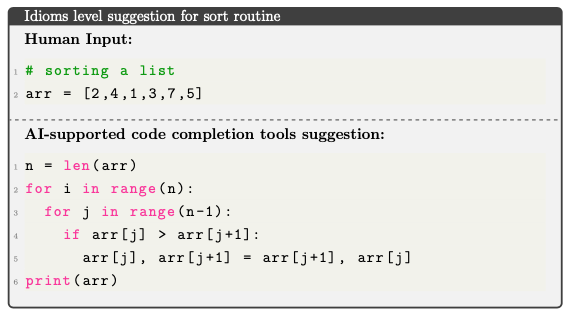
\includegraphics[width=\linewidth]{Figures/idioms.png}
    \caption{\cct{} paradigms and idioms level suggestions}
    \label{fig:idioms}
\end{figure}

The capabilities required by a \cct{} to satisfy this level of abstraction are as follows
\begin{enumerate}
    \item Use well known paradigms and language idioms whenever possible in suggesting a solution for a programming tasks.
    \item Satisfy requirements of all the levels below paradigms and idioms in our taxonomy.
\end{enumerate}

% \begin{tcolorbox}[title=Idioms level suggestion for sort routine,boxsep=.15mm]
%     %https://tex.stackexchange.com/questions/337909/tcolorbox-tcbline-style
% \textbf{Human Input:}
% \begin{lstlisting}[language={Python}]
% # sorting a list
% arr = [2,4,1,3,7,5]
% \end{lstlisting}
% \tcbline
% \textbf{\cct{} suggestion:}
% \begin{lstlisting}[language={Python}]
% n = len(arr)
% for i in range(n):
% 	for j in range(n-1):
% 		if arr[j] > arr[j+1]:
% 			arr[j], arr[j+1] = arr[j+1], arr[j]
% print(arr)
% \end{lstlisting}
% \end{tcolorbox}